%%%%%%%%%%%%%%%%%%%%%%%%%%%%%%%%%%%%%%%%%
% baposter Landscape Poster
% LaTeX Template
% Version 1.0 (11/06/13)
%
% baposter Class Created by:
% Brian Amberg (baposter@brian-amberg.de)
%
% This template has been downloaded from:
% http://www.LaTeXTemplates.com
%
% License:
% CC BY-NC-SA 3.0 (http://creativecommons.org/licenses/by-nc-sa/3.0/)
%
%%%%%%%%%%%%%%%%%%%%%%%%%%%%%%%%%%%%%%%%%

%----------------------------------------------------------------------------------------
%	PACKAGES AND OTHER DOCUMENT CONFIGURATIONS
%----------------------------------------------------------------------------------------

\documentclass[landscape,archE,fontscale=0.29]{baposter} % Adjust the font scale/size here

%%% Start of code to add %%%
\usepackage{etoolbox}
\patchcmd\thebibliography
    {\labelsep}
    {\labelsep\itemsep=0pt\relax}
    {}
    {\typeout{Couldn't patch the command}}
%%% End of code to add %%%

\usepackage{url}
\usepackage{lipsum}

\usepackage{graphicx} % Required for including images
\graphicspath{{figures/}} % Directory in which figures are stored

\usepackage{amsmath} % For typesetting math
\usepackage{amssymb} % Adds new symbols to be used in math mode

\usepackage{booktabs} % Top and bottom rules for tables
\usepackage{enumitem} % Used to reduce itemize/enumerate spacing
\usepackage{palatino} % Use the Palatino font
\usepackage[font=small,labelfont=bf]{caption} % Required for specifying captions to tables and figures

\usepackage{multicol} % Required for multiple columns
\setlength{\columnsep}{0.5em} % Slightly increase the space between columns
\setlength{\columnseprule}{0mm} % No horizontal rule between columns

\usepackage{tikz} % Required for flow chart
\usetikzlibrary{shapes,arrows} % Tikz libraries required for the flow chart in the template

\newcommand{\compresslist}{ % Define a command to reduce spacing within itemize/enumerate environments, this is used right after \begin{itemize} or \begin{enumerate}
\setlength{\itemsep}{1pt}
\setlength{\parskip}{0pt}
\setlength{\parsep}{0pt}
}

\definecolor{lightblue}{rgb}{0.145,0.6666,1} % Defines the color used for content box headers
\definecolor{lightred}{rgb}{.94,0,.337} % Defines the color used for content box headers
\definecolor{lightsilver}{rgb}{.752,0.752,.752} % Defines the color used for content box headers
\definecolor{crimson}{rgb}{.862, 0.078,.235}

% xcui macros
\usepackage[skip=2pt]{caption}
\newcommand{\myv}{\vspace{-1mm}}
% end of xcui macros


\begin{document}

\begin{poster}
{
headerborder=closed, % Adds a border around the header of content boxes
colspacing=1em, % Column spacing
bgColorOne=white, % Background color for the gradient on the left side of the poster
bgColorTwo=white, % Background color for the gradient on the right side of the poster
borderColor=black, % Border color
headerColorOne=black, % Background color for the header in the content boxes (left side)
headerColorTwo=crimson, % Background color for the header in the content boxes (right side)
headerFontColor=white, % Text color for the header text in the content boxes
boxColorOne=white, % Background color of the content boxes
textborder=roundedleft, % Format of the border around content boxes, can be: none, bars, coils, triangles, rectangle, rounded, roundedsmall, roundedright or faded
eyecatcher=true, % Set to false for ignoring the left logo in the title and move the title left
headerheight=0.13\textheight, % Height of the header
headershape=roundedright, % Specify the rounded corner in the content box headers, can be: rectangle, small-rounded, roundedright, roundedleft or rounded
headerfont=\Large\bf\textsc, % Large, bold and sans serif font in the headers of content boxes
%textfont={\setlength{\parindent}{1.5em}}, % Uncomment for paragraph indentation
linewidth=2pt % Width of the border lines around content boxes
}
%----------------------------------------------------------------------------------------
%	TITLE SECTION
%----------------------------------------------------------------------------------------
%
%% {
\includegraphics[height=10em]{img/UniversityOfWaterloo_logo_vert_rgb.png}} % First university/lab logo on the left
{
\includegraphics[height=7.5em]{img/Cheriton_Logo.pdf}} % First university/lab logo on the left
{\bf\textsc\small{NetStore: Leveraging Network Optimizations to Improve Distributed Transaction Processing Performance}\vspace{0.1em}} % Poster title
{\vspace{-2mm}
\fontfamily{pzc}\selectfont\textsc{{\huge\textbf{\underline{Xu Cui}}, Michael Mior, Supervisors: Bernard Wong,
    Khuzaima Daudjee} \\ \fontfamily{ccr}\selectfont{David R. Cheriton School of Computer Science}}} % Author names and institution
%% {\includegraphics[height=4em]{logo.png}} % Second university/lab logo on the right

%----------------------------------------------------------------------------------------
%	OBJECTIVES
%----------------------------------------------------------------------------------------

\headerbox{Background}{name=background, column=0, row=0, height=0.70}{
%% Cloud allows sharing which increases resource utilization that in turn reduces costs. However, with increased utilization there is also reduced isolation between tenants. This is especially problematic for cloud storage systems which are highly sensitive to performance interference. Since cloud storage is often the performance bottleneck in cloud application, a lack of performance isolation can lead to unpredictable application latencies.
\textbf{Distributed Storage Systems in the Cloud}
\myv
\begin{itemize}
\item The volume of data generated has increased exponentially in the past decade.
\item Distributed storage systems are needed to store data across multiple servers.
\item This makes the network a potential performance bottleneck.
\item Cloud tenants cannot control the cloud network.
\item Application level optimizations rely only on static information (i.e. fetch data from a nearby server)
\end{itemize}

\textbf{A Datacenter Network}
\begin{center}
  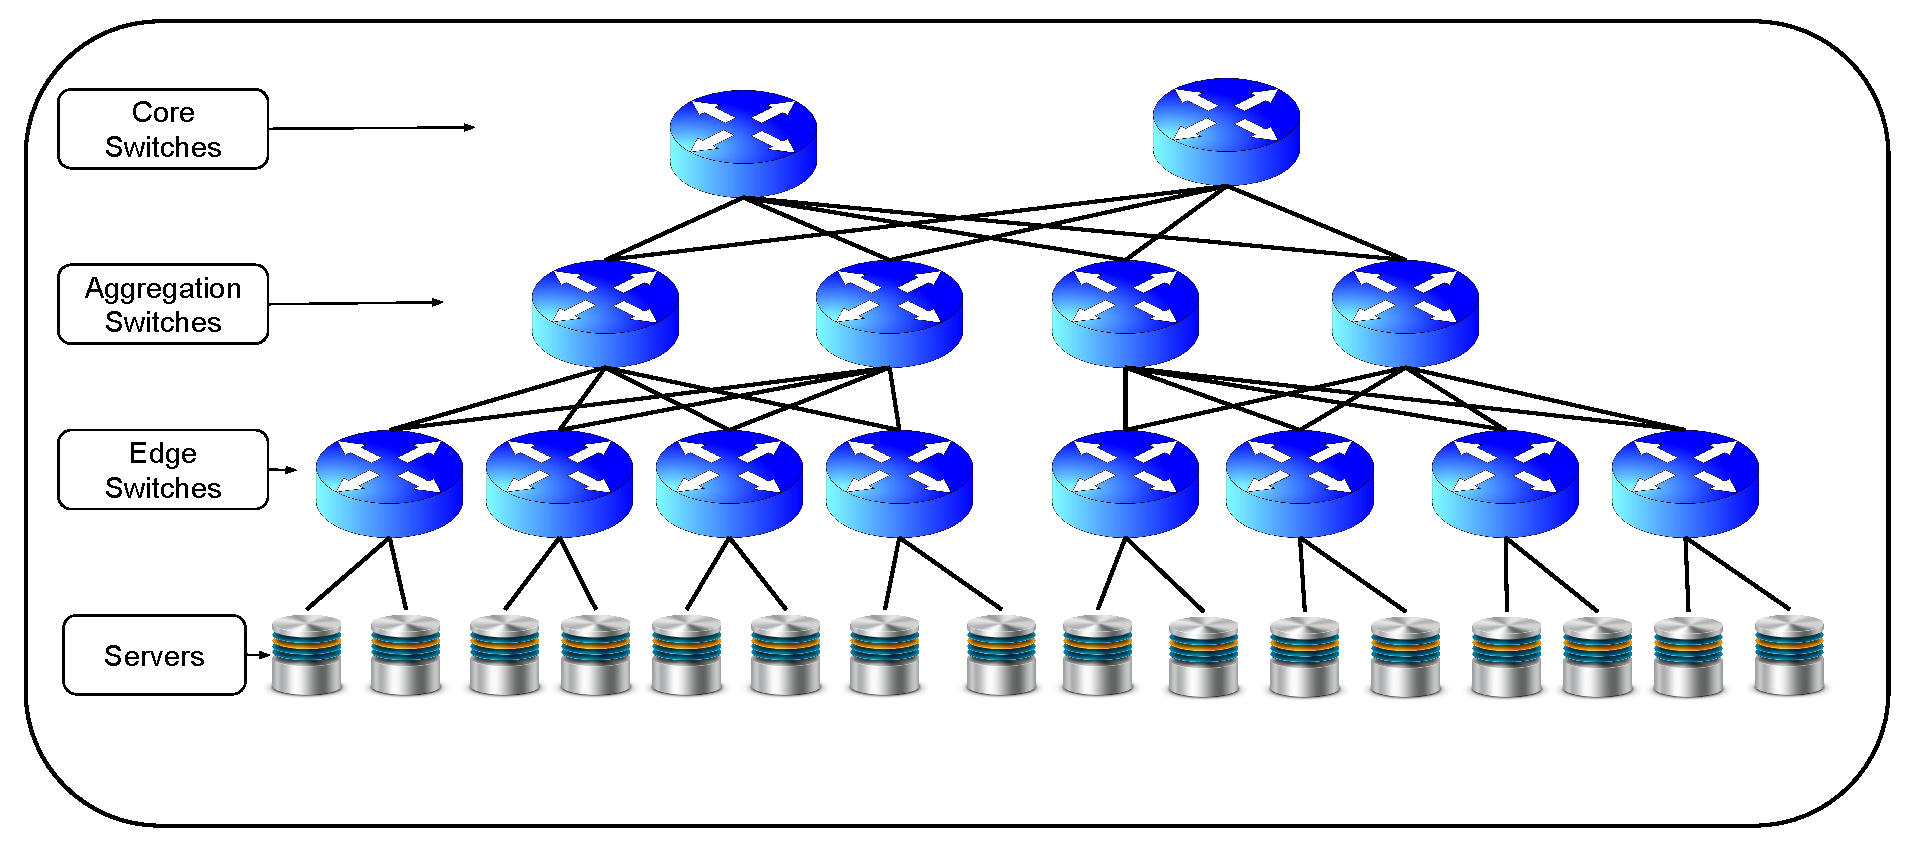
\includegraphics[scale=0.130]{img/network_arch_withOUT_pod.pdf}
  \captionof{figure}{System Overview}
\end{center}
\begin{itemize}
\item Multiple unique paths between pairs of servers.
\item Part of the network may become congested for a period of time.
\end{itemize}

%% \begin{itemize}\compresslist
%% \item[--] \scriptsize{[1] Nathan Farrington and Alexey Andreyev, Facebook's Data
  %% Center Network Architecture.}
%% \item[--] \scriptsize{[2] Greg Lindem, Make Data Useful,
  %% \url{http://www.scribd.com/doc/4970486/Make-Data-Useful-by-Greg-Linden-Amazon-com}.}
%% \end{itemize}
\vspace{0.2em} % When there are two boxes, some whitespace may need to be added if the one on the right has more content
}


\headerbox{NetStore}{name=netstore,column=1,span=2,row=0, height=0.33}{
\begin{multicols*}{2}
\vspace{1em}
A network-aware transaction processing system which applies three optimization techniques across network layer and database layer to improve performance.

\vspace{.5em}
\textbf{Least Bottlenecked Path (LBP)}
\myv
\myv
\begin{itemize}\compresslist
\item Network-aware path selection.
\end{itemize}

\textbf{Opportunistic Load Redistribution(OLR)}
\myv
\myv
\begin{itemize}\compresslist
\item  Designed to redistribute network load.
\end{itemize}

\textbf{Earliest Expected Job First (EEJF)}
\myv
\myv
\begin{itemize}\compresslist
\item Designed to further reduce the load on possibly congested links.
\end{itemize}

\vspace{3 mm}
\begin{center}
  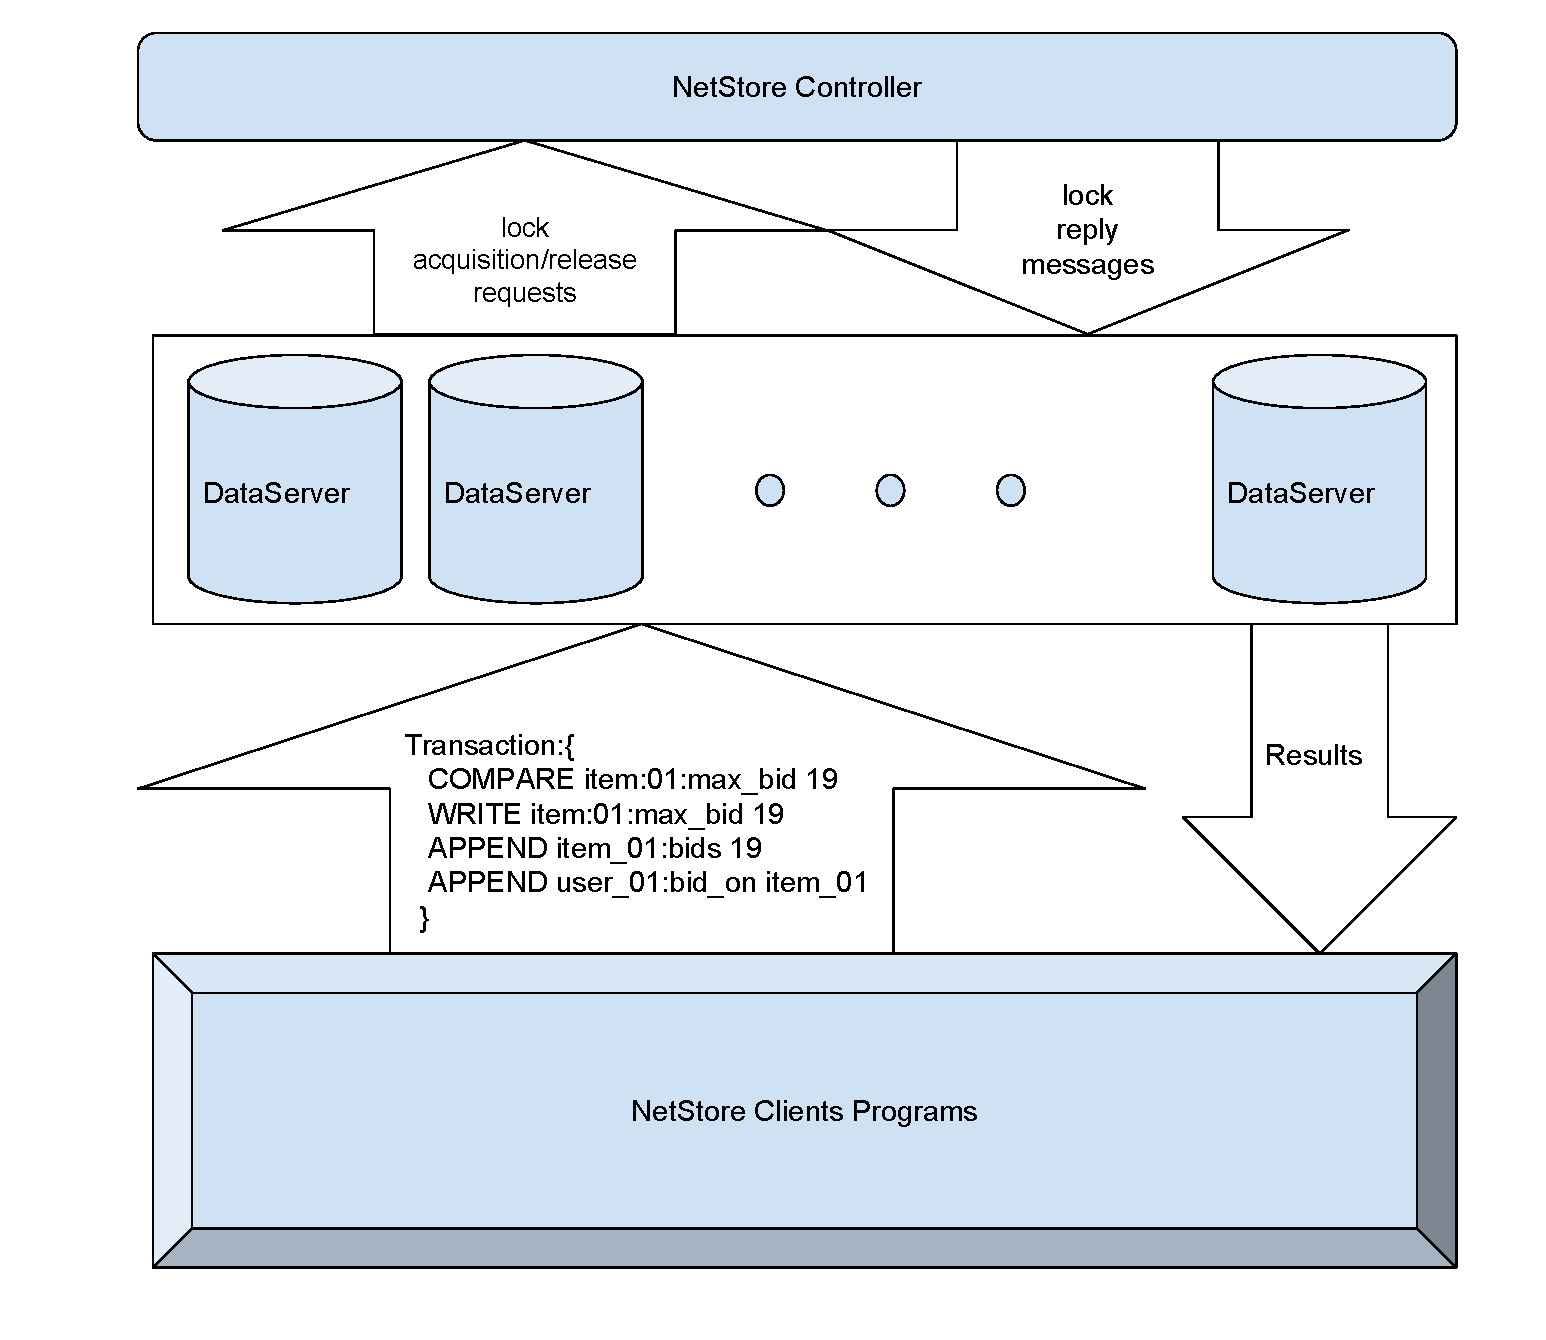
\includegraphics[scale=0.220]{img/sys_arch.pdf}
  \captionof{figure}{NetStore Architecture}
\end{center}
\end{multicols*}
\vspace{0.2em} % When there are two boxes, some whitespace may need to be added if the one on the right has more content
}


\headerbox{Opportunistic Load Redistribution}{name=olr, column=1, span=2, below=netstore, bottomaligned=background}{
  \begin{multicols}{3}
    \textbf{OLR} is a database layer optimization that effectively reduces the load on network links.
  %% \myv \myv \myv
  \begin{itemize}\compresslist
  \item OLR takes the advantage of read operation results by creating temporary replicas.
  \item Avoids complex cache eviction implementations.
  \item Avoids communication costs for cache invalidation.
  \end{itemize}
  \vfill
  \columnbreak
  \hspace{1.0em}
  \begin{center}
    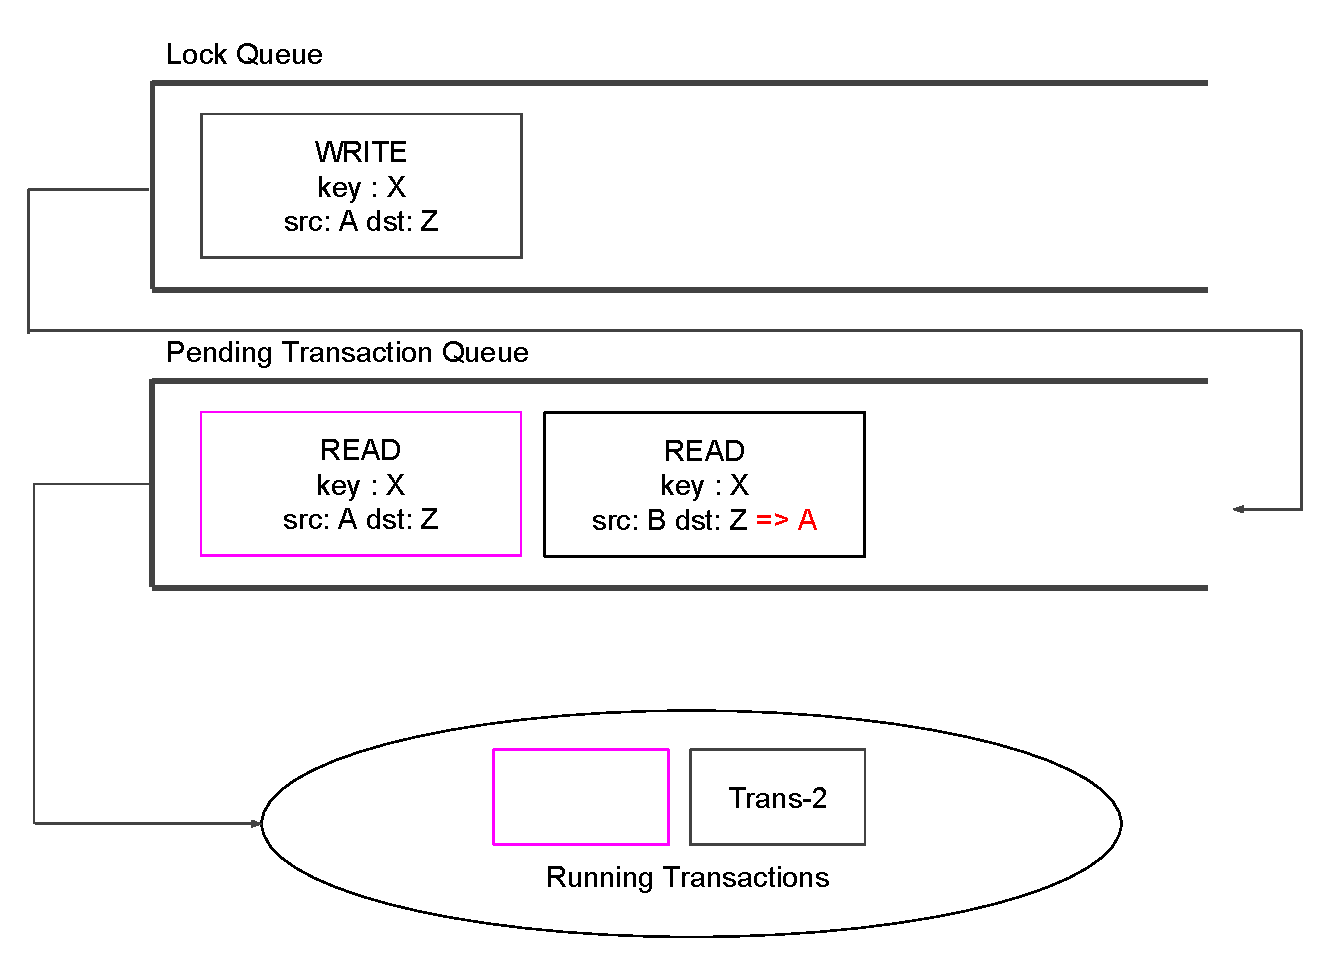
\includegraphics[scale=0.18]{img/OLR_example_1.pdf}
    \captionof{figure}{An OLR Example Part I}
  \end{center}
  \vfill
  \columnbreak
  \hspace{2.5em}
  \begin{center}
    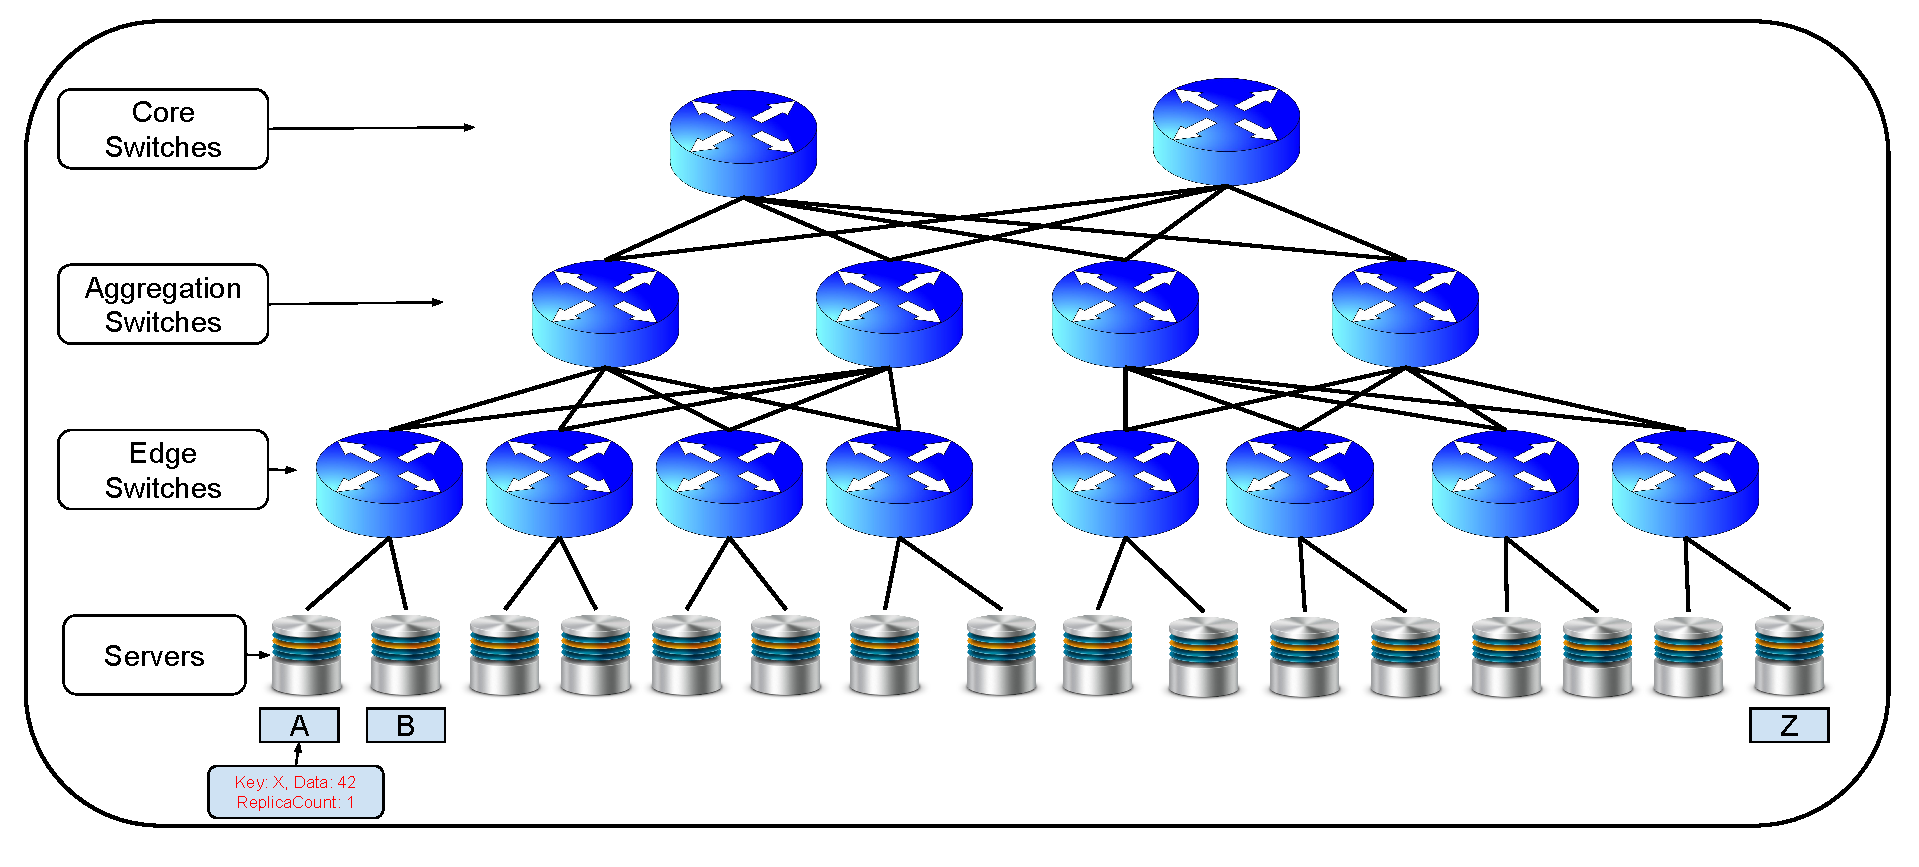
\includegraphics[scale=0.16]{img/OLR_example_2.pdf}
    \captionof{figure}{An OLR Example Part II}
  \end{center}
\end{multicols}
}

\headerbox{Least Bottlenecked Path}{name=lbp, column=3, span=1}{
  \textbf{LBP} offers network-aware path selection.
  \myv \myv \myv
  \begin{itemize}\compresslist
  \item The NetStore controller has the global view of the network.
  \item We use dynamic flow count information on each link to compute bandwidth allocation for each new flow.
  \item \textbf{LBP} Makes informed routing decisions based on dynamic flow information.
  \end{itemize}

  \begin{center}
    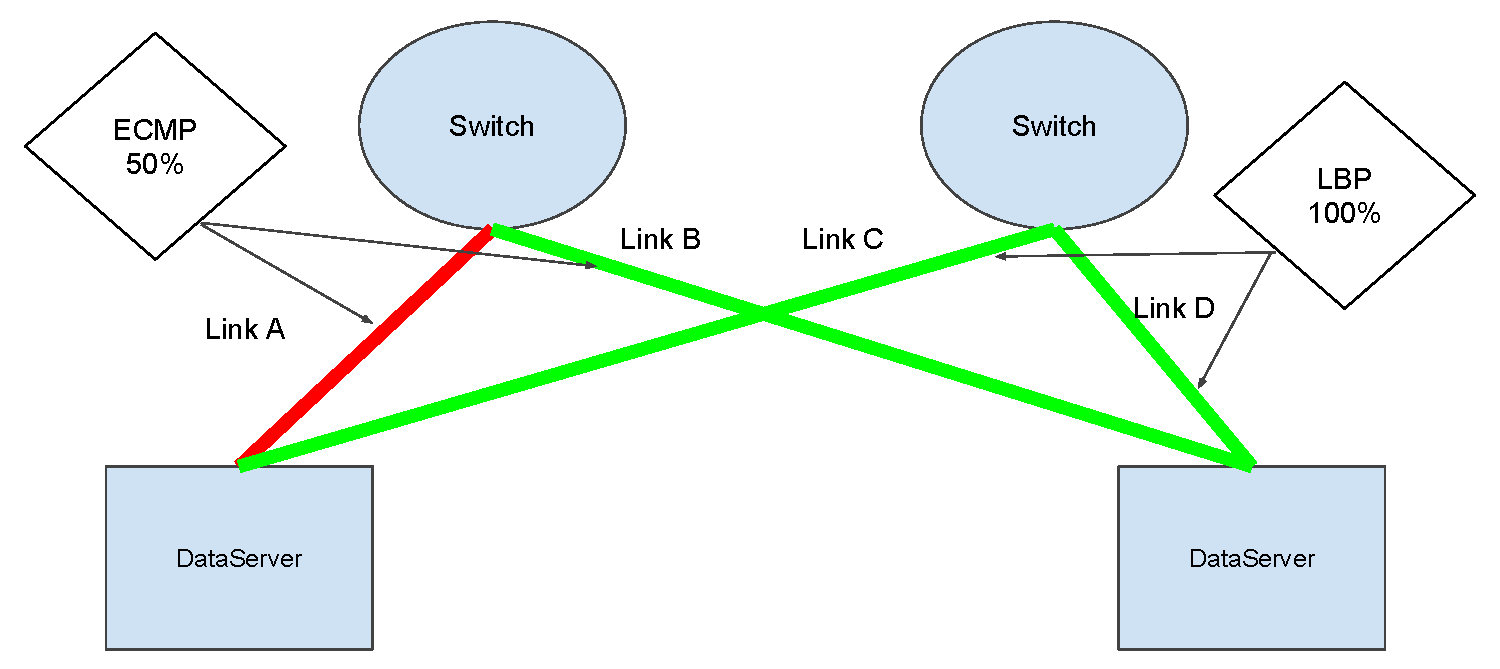
\includegraphics[scale=0.25]{img/LPB_Example.pdf}
    \captionof{figure}{A LBP Example}
  \end{center}
}

\headerbox{Earliest Expected Job First}{name=eejf, column=3, span=1,  below=lbp, bottomaligned=background}{
  \textbf{EEJF} is designed to delay the new flows that may traverse congested links.
  \begin{itemize}\compresslist
  \item We built a network-aware performance model of the underlying system.
  \item Uses this model to predict the expected completion time of a transaction.
  \item Orders the transactions using this expected completion time.
  \end{itemize}
}

\headerbox{Performance Evaluation}{name=performance, column=0, span=3,below=background, above=bottom}{
  \begin{multicols}{4}
    \begin{itemize}\compresslist
    \item We use Mininet in a 9-node cluster to emulate a multi-rooted tree topology with 1Gbps links and with a total of 64 virtual servers.
    \item We use a modified version of the RUBiS benchmark to evaluate NetStore against the Equal-Cost Multi-Path (ECMP) routing algorithm.
    \end{itemize}
    \begin{center}
      \hspace{0.5em}
      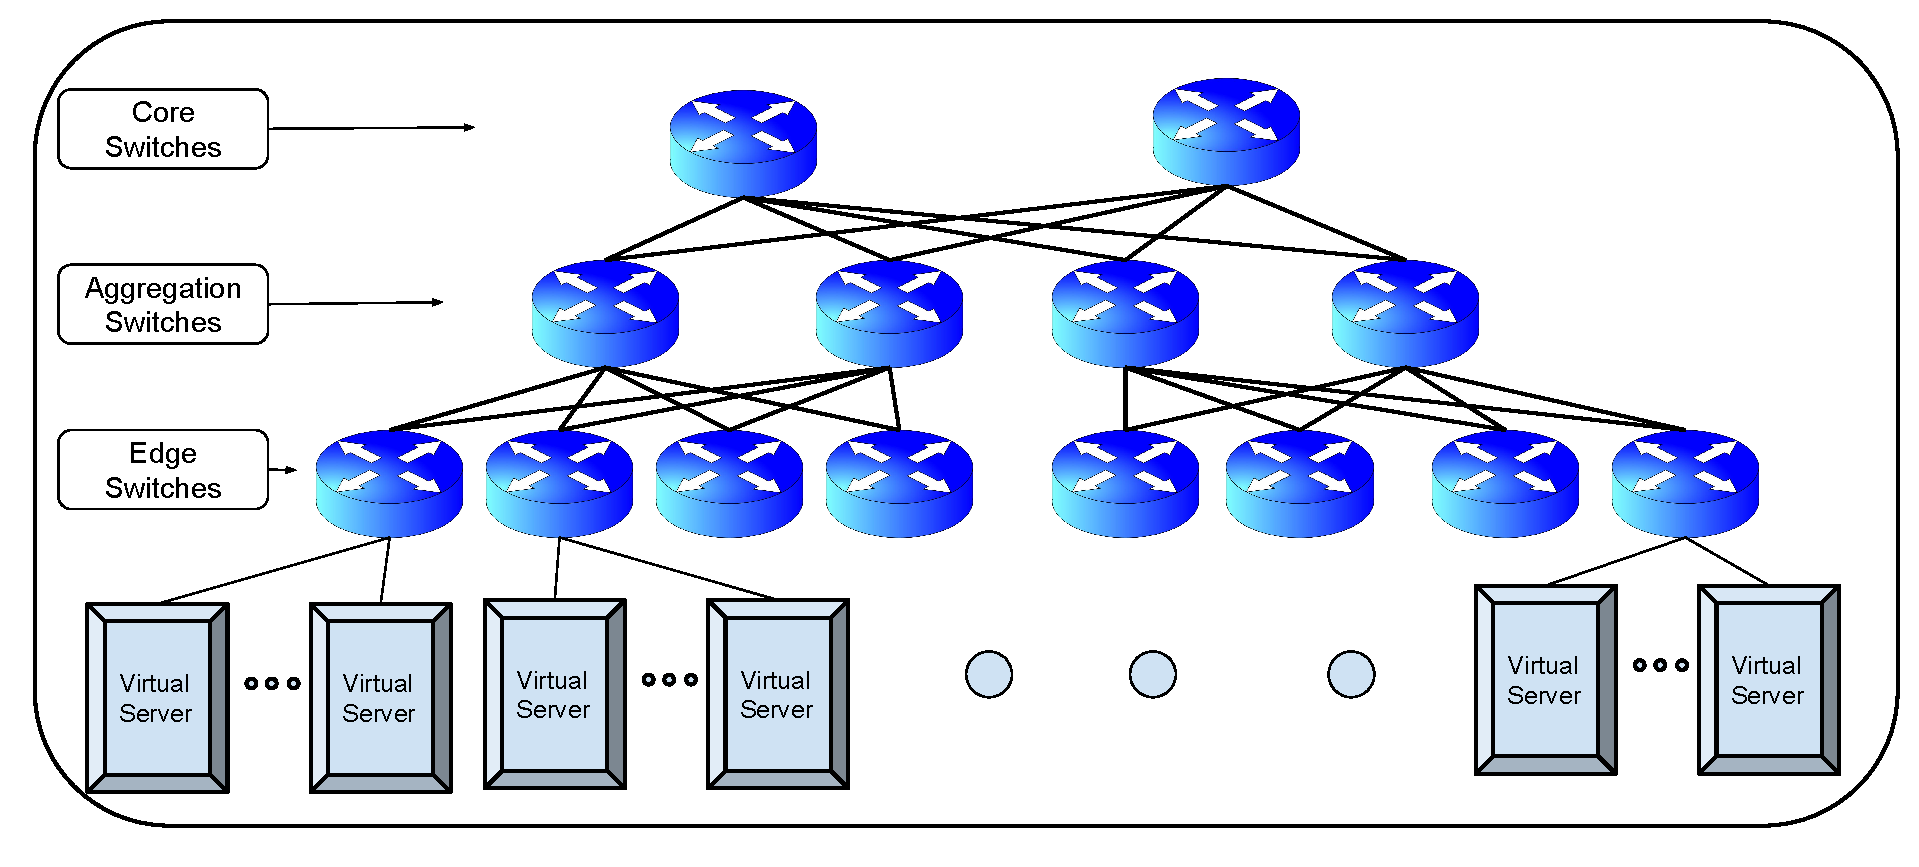
\includegraphics[scale=0.18]{img/exp_setup.pdf}
      \captionof{figure}{Testbed Network Topology Setup}
    \end{center}
    \begin{center}
      \hspace{1.0em}
      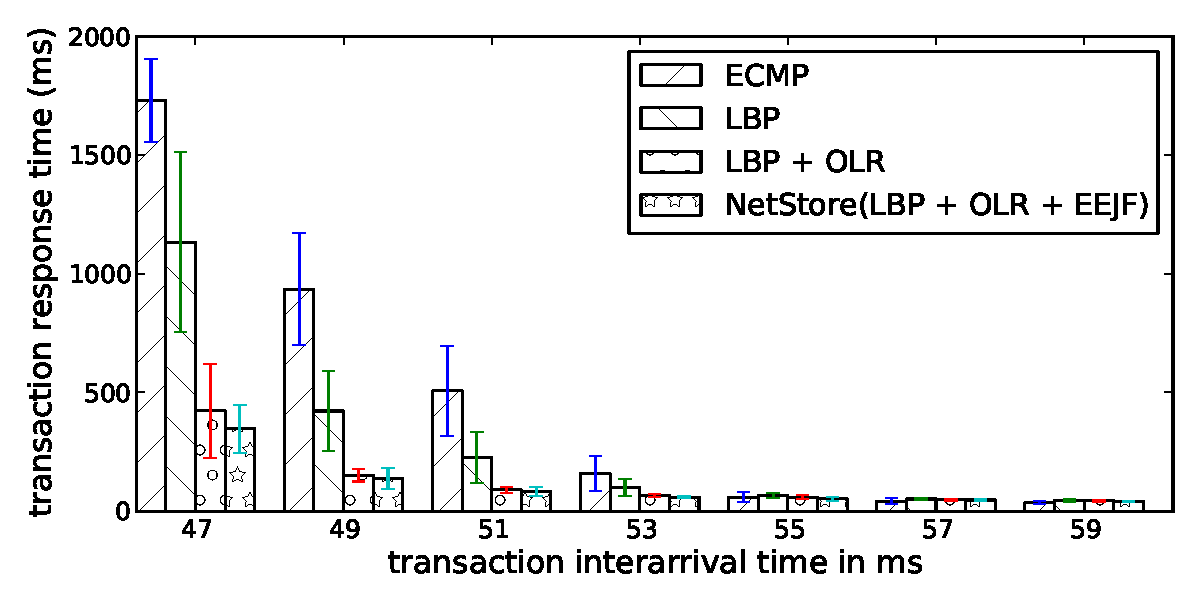
\includegraphics[scale=0.28]{img/all_bar_with_all_bars.pdf}
      \captionof{figure}{ECMP vs NetStore - Average transaction completion time.}
    \end{center}
    \vspace{1.2em}
    %% \center\textbf{Experimental Setup}
    %% \myv
    \begin{itemize}\compresslist
    \item NetStore has reduced the average transaction completion time by 85\% at an interarrival rate of 49 milliseconds.
    \item NetStore is consistently performing over 50\% better than ECMP without sacrificing throughput while the network is saturated.
    \end{itemize}
  \end{multicols}
}
\headerbox{Conclusion}{name=conclusion, column=3,below=background, above=bottom}{
  \vspace{0.1em}
  \begin{itemize}
  \item NetStore bridges the gap between network research and distributed database research to avoid transaction performance deterioration due to network saturation.
  \item NetStore uses cross-layer optimizations that rely on dynamic network information to improve transaction performance.
  %% \item NetStore significantly improves the average transaction completion times while maintaining the system throughput.
  \end{itemize}
}
\end{poster}

\end{document}
